\documentclass{article}
\usepackage[utf8]{inputenc}
\usepackage[english]{babel}
\usepackage[]{amsthm} 
\usepackage[]{amssymb} 
\usepackage{amsmath}
\DeclareMathOperator{\domain}{dom}
\usepackage{graphicx}
\usepackage{hyperref}
\usepackage{comment}
\usepackage[dvipsnames]{xcolor}
\usepackage[thinc]{esdiff}
\usepackage{tcolorbox}
\usepackage{cancel}
\usepackage{float}
\graphicspath{ {./HW1_images/} }
\newtheorem*{theorem}{Theorem}

\title{Optimization Algorithms: HW1}
\author{Lo Chun, Chou \\ R13922136}
\date\today

\begin{document}
\setlength{\parindent}{0pt}
\maketitle 

\tcbset{
    greenbox/.style={
        colback=SpringGreen!20,
        colframe=SpringGreen!80,
        coltitle=black,
        sharp corners
    },
    bluebox/.style={
        colback=SkyBlue!20,
        colframe=SkyBlue!80,
        coltitle=black,
        sharp corners
    },
    yellowbox/.style={
        colback=yellow!10,
        colframe=yellow!80,
        coltitle=black,
        sharp corners
    }
}

\section*{1}

\subsection*{(1)}

First, consider a function $g(z) = \log(1 + e^{-z})$, taking its first and second derivatives:

\begin{align*}
    g'(z) &= \frac{d}{dz} \log(1 + e^{-z}) = \frac{-e^{-z}}{1 + e^{-z}} \\
    g''(z) &= \frac{d}{dz} \left( \frac{-e^{-z}}{1 + e^{-z}} \right) = \frac{e^{-z}}{(1 + e^{-z})^2}
\end{align*}

We can see that it $g''(z)$ is nonnegative at all points, thus $g(z)$ is convex.

Now, consider $z = y_i \langle x_i, w \rangle$, and let $h(w) = \log(1 + e^{-y_i \langle x_i, w \rangle})$:

\begin{align*}
    &h: \mathbb{R}^d \to \mathbb{R} \\
    &h(w) = g(y_i \langle x_i, w \rangle)
\end{align*}

Since $g(z)$ is convex, $h(w)$ is convex.
\footnote{S. Boyd and L. Vandenberghe, \textit{Convex Optimization}, 1st ed., Cambridge University Press, 2004, p.~79.}
Also, since sum and scaling of convex functions are convex, the function $f(w)$ we're given is also convex.
\footnote{Y. Nesterov, \textit{Introductory Lectures on Convex Optimization: A Basic Course}, 1st ed., Springer, New York, NY, 2004, p.~82.}
\bigskip

Next, we compute the gradient and Hessian of $f(w)$:

\begin{align*}
    \nabla f(w) 
    &= \nabla \left( \frac{1}{n} \sum_{i = 1}^n \log \left( 1 + \mathrm{e}^{- y_i \langle x_i, w \rangle} \right) \right) \\
    &= \frac{1}{n} \sum_{i = 1}^n \nabla \log \left( 1 + \mathrm{e}^{- y_i \langle x_i, w \rangle} \right) \\
    &= \frac{1}{n} \sum_{i = 1}^n \frac{-y_i x_i e^{-y_i \langle x_i, w \rangle}}{1 + e^{-y_i \langle x_i, w \rangle}} \\
    &= \frac{1}{n} \sum_{i = 1}^n \frac{-y_i x_i}{1 + e^{y_i \langle x_i, w \rangle}}
\end{align*}

\begin{align*}
    \nabla^2 f(w) 
    &= \nabla \left( \frac{1}{n} \sum_{i = 1}^n \frac{-y_i x_i}{1 + e^{y_i \langle x_i, w \rangle}} \right) \\
    &= \frac{1}{n} \sum_{i = 1}^n \nabla \left( \frac{-y_i x_i}{1 + e^{y_i \langle x_i, w \rangle}} \right) \\
    &= \frac{1}{n} \sum_{i = 1}^n \frac{ \left( \frac{\partial}{\partial w} \left( -y_i x_i \right) \right) \left( 1 + e^{y_i \langle x_i, w \rangle} \right) - \left( -y_i x_i \right) \frac{\partial}{\partial w} \left( 1 + e^{y_i \langle x_i, w \rangle} \right) }{\left( 1 + e^{y_i \langle x_i, w \rangle} \right)^2} \\
    &= \frac{1}{n} \sum_{i = 1}^n \frac{ \left( y_i x_i \right) \frac{\partial}{\partial w} \left( 1 + e^{y_i \langle x_i, w \rangle} \right) }{\left( 1 + e^{y_i \langle x_i, w \rangle} \right)^2} \\
    &= \frac{1}{n} \sum_{i = 1}^n \frac{ \left( y_i x_i \right) \left( y_i e^{y_i \langle x_i, w \rangle} x_i \right) }{\left( 1 + e^{y_i \langle x_i, w \rangle} \right)^2} \\
    &= \frac{1}{n} \sum_{i = 1}^n \frac{ e^{y_i \langle x_i, w \rangle} x_i x_i^T }{\left( 1 + e^{y_i \langle x_i, w \rangle} \right)^2} \\
\end{align*}

Since every $x_i x_i^T$ is positive semidefinite, and is multiplied by a positive value $\frac{e^{y_i \langle x_i, w \rangle}}{(1 + e^{y_i \langle x_i, w \rangle})^2}$, the average of them, which is the Hessian $\nabla^2 f(w)$, is positive semidefinite.
\bigskip

By the following theorem
\footnote{Y. Nesterov, \textit{Introductory Lectures on Convex Optimization: A Basic Course}, 1st ed., Springer, New York, NY, 2004, p.~58.},
we can derive the Lipschitz constant $L$ of $\nabla f(w)$:

\begin{tcolorbox}[greenbox, title = Theorem 2.1.6]
    Two times continuously differentiable function $f$ belongs to $\mathsf{F}^{2,1}_L(\mathbb{R}^n)$ 
    \begin{align*}
        \Leftrightarrow 0 \preceq \nabla^2 f(x) \preceq L I_n \quad \forall x \in \mathbb{R}^n
    \end{align*}
\end{tcolorbox}

This means that the eigenvalues of the Hessian should be in the range of $[0, L]$,
and we could find $L$ by finding the maximum eigenvalue of the Hessian.
\bigskip

Observe the structure of the Hessian, the scalar of $x_i x_i^T$ is:

\begin{align*}
    \frac{ e^{y_i \langle x_i, w \rangle} }{\left( 1 + e^{y_i \langle x_i, w \rangle} \right)^2} \in (0, \frac{1}{4}]
\end{align*}

Where $\frac{1}{4}$ happens when $y_i \langle x_i, w \rangle = 0$.
\bigskip

Thus, $L = \frac{1}{4n} \lambda_{max} (\sum_{i = 1}^n x_i x_i^T)$
\bigskip

Then we could use the following scheme
\footnote{Y. Nesterov, \textit{Introductory Lectures on Convex Optimization: A Basic Course}, 1st ed., Springer, New York, NY, 2004, p.~76.} 
to solve this optimization problem, since this scheme ($2.2.6$) is optimal for unconstrained minimization of the functions from $\mathsf{S}^{1,1}_{\mu, L}(\mathbb{R}^n), \ \mu \geq 0$
\footnote{Y. Nesterov, \textit{Introductory Lectures on Convex Optimization: A Basic Course}, 1st ed., Springer, New York, NY, 2004, p.~77.}

\begin{figure}[H]
    \centering
    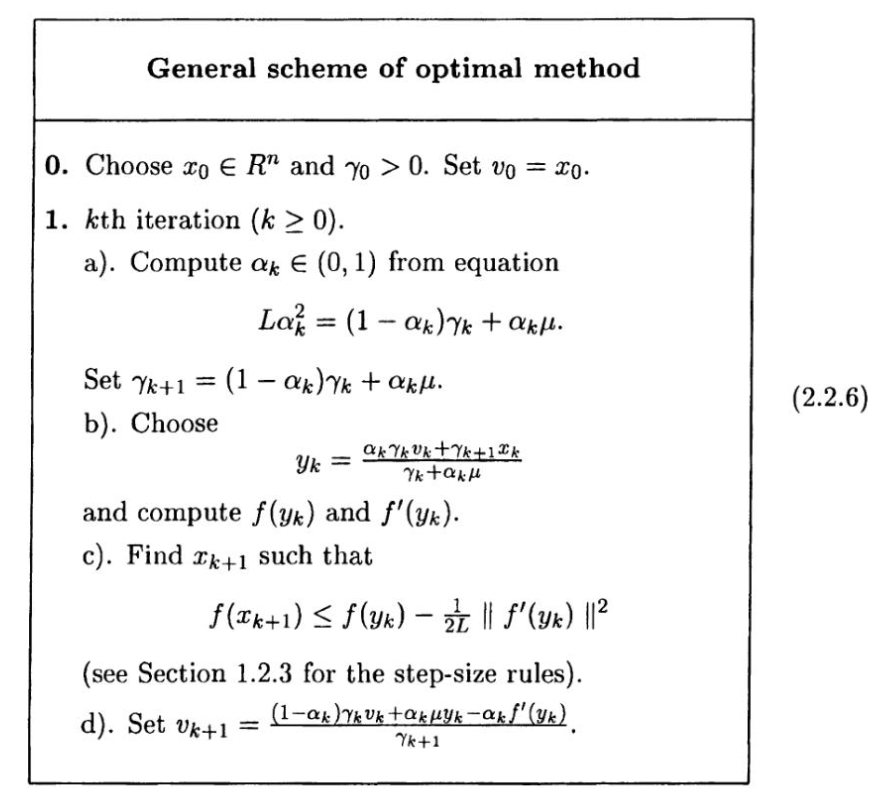
\includegraphics[width = 0.7\textwidth]{general_scheme_of_optimal_method.png}
\end{figure}

In our case, we set $\mu = 0$ since we cannot guarantee strongly convexity, and $L$ as the Lipschitz constant we just derived.
\bigskip

By Theorem $2.2.2$
\footnote{Y. Nesterov, \textit{Introductory Lectures on Convex Optimization: A Basic Course}, 1st ed., Springer, New York, NY, 2004, p.~77.}
, we have:

\begin{align*}
    f(x_k) - f^* \leq L \min \left\{ \left(1 - \sqrt{\frac{\mu}{L}}\right)^k, \frac{4}{(k+2)^2} \right\} \Vert x_0 - x^* \Vert^2
\end{align*}

Since we have $\mu = 0$, we can write the above optimization error guarantee of our problem as:

\begin{align*}
    f(w_k) - f^* \leq \frac{4L \Vert w_0 - w^* \Vert^2}{(k+2)^2} 
\end{align*}

\section*{2}

\subsection*{(1)}

Given a twice differentiable function $\varphi: \mathbb{R}^d \to [- \infty, \infty]$, 
assume that it is logarithmically homogeneous, 
then by the definition, the following holds:

\begin{align*}
    \varphi ( \gamma x ) = \varphi (x) - \log \gamma, \quad \forall x \in \mathbb{R}^d, \gamma > 0 \tag{1}
\end{align*}

\textcolor{blue}{\underline{Claim: $\langle \nabla \varphi (x), x \rangle = - 1$ } }
\bigskip

To derive the first equation, we first define the following:

\begin{align*}
    F(\gamma) = \textcolor{orange}{\varphi (\gamma x)}
\end{align*}

Then the original equation $(1)$ would become:

\begin{align*}
    F(\gamma) = \textcolor{Green}{\varphi (x) - \log \gamma}
\end{align*}

Taking the derivative w.r.t. $\gamma$ on both sides, we get:

\begin{align*}
    \frac{dF}{d\gamma} &= \frac{d}{d\gamma} \textcolor{orange}{\varphi (\gamma x)} = \nabla \varphi (\gamma x) \cdot x = \langle \nabla \varphi (\gamma x), x \rangle \tag{2}\\
    \frac{dF}{d\gamma} &= \frac{d}{d\gamma} (\textcolor{Green}{\varphi (x) - \log \gamma}) = - \frac{1}{\gamma} \tag{3}
\end{align*}

Thus by $(2)$ and $(3)$, we have:

\begin{align*}
    \langle \nabla \varphi (\gamma x), x \rangle = - \frac{1}{\gamma}
\end{align*}
Then by plugging in $\gamma = 1$, we have:

\begin{align*}
    \langle \nabla \varphi (x), x \rangle = - 1 \qquad \square
\end{align*}

\textcolor{blue}{\underline{Claim: $\nabla \varphi (x) = - \nabla^2 \varphi ( x ) x$ } }
\bigskip

From the previous part, we have:

\begin{align*}
    \nabla \varphi (x)^T x = - 1
\end{align*}

Compute the gradient of both sides, for the left hand side, we have:

\begin{align*}
    \textcolor{orange}{\nabla(}\nabla \varphi (x)^T x\textcolor{orange}{)}
    &= \textcolor{orange}{\nabla (}\nabla \varphi (x)\textcolor{orange}{)}^T x + \nabla \varphi (x)^T \textcolor{orange}{\nabla} x  \\
    &= \nabla^2 \varphi (x) x + \nabla \varphi (x)^T \nabla x  \\
\end{align*}

For the right hand side, we have:

\begin{align*}
    \nabla (- 1) = 0
\end{align*}

Thus we have:

\begin{align*}
    &\nabla^2 \varphi (x) x + \nabla \varphi (x)^T \nabla x = 0 \\
    \Rightarrow &\nabla \varphi (x)^T \nabla x = - \nabla^2 \varphi (x) x \\
    \Rightarrow &\nabla \varphi (x)^T I_d = - \nabla^2 \varphi (x) x \\
    \Rightarrow &\nabla \varphi (x) = - \nabla^2 \varphi (x) x \qquad \square
\end{align*}

\textcolor{blue}{\underline{Claim: $\langle x, \nabla^2 \varphi (x) x \rangle = 1$ } }
\bigskip

From the previous part, we have:

\begin{align*}
    \nabla \varphi (x) = - \nabla^2 \varphi (x) x
\end{align*}

Multiply both sides by $x^T$, we have:

\begin{align*}
    x^T \nabla \varphi (x) = - x^T \nabla^2 \varphi (x) x
\end{align*}

Which is equivalent to the following by using $\langle \nabla \varphi (x), x \rangle = - 1$:

\begin{align*}
    \langle x, \nabla^2 \varphi (x) x \rangle = - \langle x, \nabla \varphi (x) \rangle = (-1) \times (-1) = 1 \qquad \square
\end{align*}

\subsection*{(2)}

Suppose that $\varphi: \mathbb{R}^d \to [- \infty, \infty]$ is a twice differentiable function, 
and is strictly convex and logarithmically homogeneous, then the following holds by the definition:

\begin{align*}
    &\nabla^2 \varphi (x) > 0 \quad \forall x \in \mathbb{R}^d \\
    &\varphi ( \gamma x ) = \varphi (x) - \log \gamma, \quad \forall x \in \mathbb{R}^d, \gamma > 0.
\end{align*}

Also, we have the following properties from the previous subsection:

\begin{align*}
    \langle \nabla \varphi (x), x \rangle = - 1 \tag{1}\\
    \nabla \varphi (x) = - \nabla^2 \varphi ( x ) x \tag{2}\\
    \langle x, \nabla^2 \varphi (x) x \rangle = 1 \tag{3}
\end{align*}

\textcolor{blue}{\underline{Claim: $\nabla^2 \varphi ( x ) \geq \nabla \varphi ( x ) \left( \nabla \varphi (x) \right)^T , \quad \forall x \in \operatorname{dom}\, \varphi $} }
\bigskip

The claim is equivalent to proving that:

\begin{align*}
    \nabla^2 \varphi ( x ) - \nabla \varphi ( x ) \left( \nabla \varphi (x) \right)^T \succeq 0
\end{align*}

where $\succeq 0$ denotes positive semidefinite.

Let $z$ be any vector in $\mathbb{R}^d$, then we have:

\begin{align*}
    z^T \left( \nabla^2 \varphi ( x ) - \nabla \varphi ( x ) \left( \nabla \varphi (x) \right)^T \right) z
    &= z^T \nabla^2 \varphi ( x ) z - z^T \nabla \varphi ( x ) \left( \nabla \varphi (x) \right)^T z \\
    &= z^T \nabla^2 \varphi ( x ) z - \left( \nabla \varphi ( x )^T z \right)^2 \tag{*}\\
\end{align*}

\textbf{\underline{Case 1: $x = z$}}
\bigskip

If $x = z$, then $(*)$ becomes the following using \textcolor{orange}{$(1)$} and \textcolor{Green}{$(2)$}:

\begin{align*}
    z^T \left( \nabla^2 \varphi ( x ) - \nabla \varphi ( x ) \left( \nabla \varphi (x) \right)^T \right) z 
    &= z^T \textcolor{Green}{\nabla^2 \varphi ( x ) x} - (\textcolor{orange}{\langle \nabla \varphi ( x ), x \rangle})^2 \\
    &= x^T \textcolor{Green}{(- \nabla \varphi ( x ))} - (\textcolor{orange}{-1})^2 \\
    &= x^T (- \nabla \varphi ( x )) - 1 \\
    &= - \textcolor{orange}{\langle \nabla \varphi ( x ), x \rangle} - 1 \\
    &= - \textcolor{orange}{(-1)} - 1 \\
    &= 0 \geq 0 
\end{align*}

\textbf{\underline{Case 2: $x \neq z$}}
\bigskip

Using \textcolor{Green}{$(2)$} to replace $\nabla \varphi (x)$ with $- \nabla^2 \varphi ( x ) x$ in $(*)$, 
and using the fact that $(\nabla^2 \varphi ( x ))^T = \nabla^2 \varphi ( x )$ (the Hessian is symmetric):

\begin{align*}
    z^T \left( \nabla^2 \varphi ( x ) - \nabla \varphi ( x ) \left( \nabla \varphi (x) \right)^T \right) z 
    &= z^T \nabla^2 \varphi ( x ) z - \left( \textcolor{Green}{\nabla \varphi ( x )}^T z \right)^2 \\
    &= z^T \nabla^2 \varphi ( x ) z - \left( \textcolor{Green}{(- \nabla^2 \varphi ( x ) x)}^T z \right)^2 \\
    &= z^T \nabla^2 \varphi ( x ) z - \left( - \underbrace{x^T}_{A^T} \underbrace{(\nabla^2 \varphi ( x ))^T z }_{B} \right)^2 \\
    &= z^T \nabla^2 \varphi ( x ) z - \underbrace{[(\nabla^2 \varphi ( x ))^T z]^T x x^T [(\nabla^2 \varphi ( x ))^T z]}_{B^TAA^TB} \\
    &= z^T \nabla^2 \varphi ( x ) z - [\textcolor{blue}{x^T (\nabla^2 \varphi ( x ))^T z}]^T [\textcolor{blue}{x^T (\nabla^2 \varphi ( x ))^T z}] \\
    &= z^T \nabla^2 \varphi ( x ) z - ||\textcolor{blue}{x^T (\nabla^2 \varphi ( x ))^T z}||^2 \\
    &= z^T \nabla^2 \varphi ( x ) z - ||x^T (\nabla^2 \varphi ( x )) z||^2 
\end{align*}

Let $H = \nabla^2 \varphi ( x )$, then the above expression is equivalent to:

\begin{align*}
    z^T H z - (x^T H z)^2
\end{align*}

Let's first check that we can define the function 
\begin{align*}
    h: \mathbb{R}^d \times  \mathbb{R}^d \to \mathbb{R}, \quad h(u, v) = u^T H v
\end{align*}

as the inner product on $\mathbb{R}^d$.
\footnote{H. Amann and J. Escher, \textit{Analysis I}, 1st ed., Birkhäuser Basel, 2005, p.~153.}
\bigskip

Using the fact that we assumed that $\nabla^2 \varphi (x) > 0$, so $H$ is positive definite, 
thus by theorem
\footnote{``Square root of a matrix'', Wikipedia, \url{https://en.wikipedia.org/wiki/Square_root_of_a_matrix}}, 
there exists a one and only one positive definite matrix $H^{1/2}$ (also symmetric) such that $H = H^{1/2} H^{1/2}$.

\begin{itemize}
    \item \textbf{Symmetry:} For any $u, v \in \mathbb{R}^d$, we have:
    \begin{align*}
        h(u, v) 
        &= u^T H v \\
        &= u^T H^{1/2} H^{1/2} v \\
        &= (H^{1/2} u)^T (H^{1/2} v) \\
        &= (H^{1/2} v)^T (H^{1/2} u) \\
        &= v^T H^{1/2} H^{1/2} u \\
        &= v^T H u \\
        &= h(v, u)
    \end{align*}
    \item \textbf{Linearity:} For any $\lambda, \mu \in \mathbb{R}$ and $t, u, v \in \mathbb{R}^d$, we have:
    \begin{align*}
        h(t, \lambda u + \mu v) 
        &= t^T H (\lambda u + \mu v) \\
        &= t^T H (\lambda u + \mu v) \\
        &= t^T H (\lambda u) + t^T H (\mu v) \\
        &= \lambda t^T H u + \mu t^T H v \\
        &= \lambda h(t, u) + \mu h(t, v)
    \end{align*}
    \item \textbf{Positive definiteness:} For any $u \in \mathbb{R}^d$, we have:
    \begin{align*}
        h(u, u) = u^T H u > 0 \quad \text{since $H$ is positive definite}
    \end{align*}
\end{itemize}
\footnote{I later found that we have 
"A function $\langle \cdot, \cdot \rangle : \mathbb{R}^n \times \mathbb{R}^n \to \mathbb{R}$ 
is an inner product on $\mathbb{R}^n$ if and only if there exists a symmetric positive-definite matrix $\mathbf{M}$ 
such that $\langle x, y \rangle = x^\top \mathbf{M} y$ for all $x, y \in \mathbb{R}^n$."
on ``Inner product space'', Wikipedia, \url{https://en.wikipedia.org/wiki/Inner_product_space}}

Therefore, we have:

\begin{align*}
    z^T H z - (x^T H z)^2 
    &= \langle z, z \rangle_H - \langle x, z \rangle_H^2 \\
\end{align*}

Using the Cauchy-Schwarz inequality
\footnote{H. Amann and J. Escher, \textit{Analysis I}, 1st ed., Birkhäuser Basel, 2005, p.~154.}:
\bigskip

\begin{tcolorbox}[greenbox, title = Cauchy-Schwarz inequality]
    Let $(E, (\cdot \mid \cdot))$ be an inner product space. Then  
    \begin{align*}
        |(x \mid y)|^2 \leq (x \mid x)(y \mid y), \qquad x,y \in E
    \end{align*}
\end{tcolorbox}

We can derive the later equation using the fact that:

\begin{align*}
    \langle x, x \rangle_H = x^T H x = x^T \nabla^2 \varphi ( x ) x = 1
\end{align*}

(this is because property $(3)$)

So we have:

\begin{align*}
    \langle x, z \rangle_H^2 
    &\leq \langle x, x \rangle_H \langle z, z \rangle_H \\
    &= 1 \times \langle z, z \rangle_H \\
    &= \langle z, z \rangle_H
\end{align*}

Thus we have:

\begin{align*}
    z^T H z - (x^T H z)^2 \geq 0 \qquad \square
\end{align*}

\subsection*{(3)}

We need to prove the following equivalence:

\begin{align*}
    & \text{(1)} \quad e^{-\varphi(x)} \text{ is concave} \\
    \iff \quad & \text{(2)} \quad \varphi(y) \geq \varphi(x) - \log(1 - \langle \nabla \varphi(x), y - x \rangle), \quad \forall x, y \in \operatorname{dom}(\varphi) \\
    \iff \quad & \text{(3)} \quad \nabla^2 \varphi(x) \succeq \nabla \varphi(x) \nabla \varphi(x)^\top, \quad \forall x \in \operatorname{dom}(\varphi)
\end{align*}

\textbf{\underline{(1) $\implies$ (2)}}
\bigskip

Let $f: \mathbb{R}^d \to \mathbb{R}$ be defined as $f(x) = e^{-\varphi(x)}$.
\bigskip

Suppose that $f(x) = e^{-\varphi(x)}$ is concave, then by the definition of concavity
\footnote{Y. Nesterov, \textit{Introductory Lectures on Convex Optimization: A Basic Course}, 1st ed., Springer, New York, NY, 2004, p.~52.}:

\begin{tcolorbox}[bluebox, title = Convex]
    A continuously differentiable function $f(x)$ is called convex on $\mathbb{R}^n$ if for any $x, y \in \mathbb{R}^n$, we have:
    \begin{align*}
        f(y) \geq f(x) + \langle \nabla f(x), y - x \rangle
    \end{align*}
    If $-f(x)$ is convex, then $f(x)$ is concave.
\end{tcolorbox}

this means that our assumption is equivalent to saying that $-e^{-\varphi(x)}$ is convex. 
Let $g(x) = -f(x) = -e^{-\varphi(x)}$ a convex function, 
using the fact that:
\begin{align*}
    \nabla g(x) = \frac{d}{dx} (-e^{-\varphi(x)}) = e^{-\varphi(x)} \nabla \varphi(x)
\end{align*}

we have the following:
\bigskip

For any $x, y \in \mathbb{R}^d$:

\begin{align*}
    &g(y) \geq g(x) + \langle \nabla g(x), y - x \rangle \\
    \Rightarrow \ &-e^{-\varphi(y)} \geq -e^{-\varphi(x)} + \langle e^{-\varphi(x)} \nabla \varphi(x), y - x \rangle \\
    \Rightarrow \ &e^{-\varphi(y)} \leq e^{-\varphi(x)} - e^{-\varphi(x)} \langle \nabla \varphi(x), y - x \rangle \\
    \Rightarrow \ &e^{-\varphi(y)} \leq e^{-\varphi(x)} (1 - \langle \nabla \varphi(x), y - x \rangle) \\
    \Rightarrow \ &- \varphi(y) \leq -\varphi(x) + \log (1 - \langle \nabla \varphi(x), y - x \rangle) \\
    \Rightarrow \ &\varphi(y) \geq \varphi(x) - \log (1 - \langle \nabla \varphi(x), y - x \rangle)
\end{align*}

\textbf{\underline{(2) $\implies$ (3)}}
\bigskip

Suppose $(2)$ holds, so we have:

\begin{align*}
    \varphi(y) \geq \varphi(x) - \log (1 - \langle \nabla \varphi(x), y - x \rangle), \quad \forall x, y \in \operatorname{dom}(\varphi)
\end{align*}

By plugging in $y = x + h \ (h = y - x)$, with $||h|| \rightarrow 0$, we have:

\begin{align*}
    \varphi(x + h) \geq \varphi(x) - \log (1 - \langle \nabla \varphi(x), h \rangle) \tag{1}
\end{align*}

Then by using the second-order approximation
\footnote{Y. Nesterov, \textit{Introductory Lectures on Convex Optimization: A Basic Course}, 1st ed., Springer, New York, NY, 2004, p.~19.}:

\begin{tcolorbox}[bluebox, title = Second-order approximation]
    Let $f$ be twice differentiable at $\bar{x}$. Then
    \begin{align*}
        f(y) = f(\bar{x}) + \langle \nabla f(\bar{x}), y - \bar{x} \rangle + \frac{1}{2} \langle\nabla^2 f(\bar{x}) (y - \bar{x}), y - \bar{x} \rangle + o(||y - \bar{x}||^2)
    \end{align*}
\end{tcolorbox}

Since $\varphi$ is twice differentiable on its domain, we have:

\begin{align*}
    \varphi(x + h) = \varphi(x) + \langle \nabla \varphi(x), h \rangle + \frac{1}{2} \langle\nabla^2 \varphi(x) h, h \rangle + o(||h||^2) \tag{2}
\end{align*}

Combining $(1)$ and $(2)$, we have:

\begin{align*}
    &\textcolor{orange}{\varphi(x)} + \langle \nabla \varphi(x), h \rangle + \frac{1}{2} \langle\nabla^2 \varphi(x) h, h \rangle + o(||h||^2) 
    \geq \textcolor{orange}{\varphi(x)} - \log (1 - \langle \nabla \varphi(x), h \rangle) \\
    \Rightarrow \ &\langle \nabla \varphi(x), h \rangle + \frac{1}{2} \langle\nabla^2 \varphi(x) h, h \rangle + o(||h||^2)  \geq - \textcolor{Green}{\log (1 - \langle \nabla \varphi(x), h \rangle)}  \\
    \Rightarrow \ &\langle \nabla \varphi(x), h \rangle + \frac{1}{2} \langle\nabla^2 \varphi(x) h, h \rangle + o(||h||^2)  \geq - \textcolor{Green}{(-\sum_{n=1}^{\infty} \frac{\langle \nabla \varphi(x), h \rangle^n}{n})}  \\
    \Rightarrow \ &\textcolor{blue}{\langle \nabla \varphi(x), h \rangle} + \frac{1}{2} \langle\nabla^2 \varphi(x) h, h \rangle + o(||h||^2)  \geq \textcolor{blue}{\langle \nabla \varphi(x), h \rangle} + \sum_{n=2}^{\infty} \frac{\langle \nabla \varphi(x), h \rangle^n}{n}  \\
    \Rightarrow \ &\frac{1}{2} \langle\nabla^2 \varphi(x) h, h \rangle + o(||h||^2)  \geq \sum_{n=2}^{\infty} \frac{\langle \nabla \varphi(x), h \rangle^n}{n}  \\
    \Rightarrow \ &\frac{1}{2} \langle\nabla^2 \varphi(x) h, h \rangle + o(||h||^2)  \geq \frac{\langle \nabla \varphi(x), h \rangle^2}{2} + \frac{\langle \nabla \varphi(x), h \rangle^3}{3} + \cdots \tag{*}\\
\end{align*}

Examine the terms on the right hand side by Cauchy-Schwarz inequality:

\begin{align*}
    \frac{(\textcolor{orange}{\langle \nabla \varphi(x), h \rangle})^3}{3} 
    &\textcolor{orange}{\leq} \frac{(\textcolor{orange}{||\nabla \varphi(x)|| \cdot ||h||})^3}{3} \\
\end{align*}

Since $||h|| \rightarrow 0$ by our assumption, we can write:

\begin{align*}
    \frac{\langle \nabla \varphi(x), h \rangle^2}{2} + \frac{\langle \nabla \varphi(x), h \rangle^3}{3} + \cdots = o(||h||^2)
\end{align*}

Substituting this bound back into $(*)$, we have:

\begin{align*}
    &\frac{1}{2} \langle\nabla^2 \varphi(x) h, h \rangle + o(||h||^2)  \geq \frac{\langle \nabla \varphi(x), h \rangle^2}{2} + o(||h||^2) \\
    \Rightarrow \ & \ \frac{1}{2} \langle\nabla^2 \varphi(x) h, h \rangle  \geq \frac{\langle \nabla \varphi(x), h \rangle^2}{2} \\
    \Rightarrow \ & \ \langle\nabla^2 \varphi(x) h, h \rangle  \geq \langle \nabla \varphi(x), h \rangle^2 \\
    \Rightarrow \ & \ (\nabla^2 \varphi(x) h)^T h \geq (\nabla \varphi(x)^T h)^T (\nabla \varphi(x)^T h) \\
    \Rightarrow \ & \ h^T \textcolor{blue}{(\nabla^2 \varphi(x))^T} h \geq h^T \textcolor{blue}{\nabla \varphi(x) (\nabla \varphi(x))^T} h \\
    \Rightarrow \ & \ h^T \textcolor{blue}{((\nabla^2 \varphi(x))^T - \nabla \varphi(x) (\nabla \varphi(x))^T)} h \geq 0 \\
    \Rightarrow \ & \ \nabla^2 \varphi(x) - \nabla \varphi(x) (\nabla \varphi(x))^T \succeq 0 \qquad \qquad \text{(since the Hessian is symmetric)}
\end{align*}

Thus, we have proved that:

\begin{align*}
    \nabla^2 \varphi(x) \geq \nabla \varphi(x) (\nabla \varphi(x))^T, \quad \forall x,y \in \domain \varphi
\end{align*}

\textbf{\underline{(3) $\implies$ (1)}}
\bigskip

Suppose $(3)$ holds, so we have:

\begin{align*}
    \nabla^2 \varphi(x) \geq \nabla \varphi(x) (\nabla \varphi(x))^T, \quad \forall x,y \in \domain \varphi
\end{align*}

Since we need to show that $e^{-\varphi(x)}$ is concave, similar to the previous proof, we can define $g(x) = -f(x) = -e^{-\varphi(x)} \ (\text{ where } f(x) = e^{-\varphi(x)})$,
and show that $g(x)$ is convex.
\bigskip

By theorem
\footnote{Y. Nesterov, \textit{Introductory Lectures on Convex Optimization: A Basic Course}, 1st ed., Springer, New York, NY, 2004, p.~55.}, 
we have:
\begin{tcolorbox}[greenbox, title = Theorem 2.1.4]
    Two times continuously differentiable function $f \in \mathcal{F}^2(\mathbb{R}^n)$ iff for any $x \in \mathbb{R}^n$, we have:
    \begin{align*}
        f''(x) \succeq 0
    \end{align*}
\end{tcolorbox}

Therefore, we need to show that $\nabla^2 g(x) \succeq 0$.
We derive the following using the Scalar-by-vector identity
\footnote{``Matrix calculus'', Wikipedia, \url{https://en.wikipedia.org/wiki/Matrix_calculus}}:
\bigskip

If $u = u(x)$ and $v = v(x)$ are vector functions of $x$, then:
\begin{align*}
    \nabla (u \cdot v) = (\nabla u) v^T + u^T (\nabla v)
\end{align*}

Hence, we have:

\begin{align*}
    \nabla^2 g(x) 
    &= \nabla(e^{-\varphi(x)} \nabla \varphi(x)) \\
    &= \left[ \frac{d}{dx}(e^{-\varphi(x)}) \right] (\nabla \varphi(x))^T + e^{-\varphi(x)} \nabla^2 \varphi(x) \\
    &= \textcolor{orange}{-} e^{-\varphi(x)} \textcolor{orange}{(\nabla \varphi(x))(\nabla \varphi(x))^T} + e^{-\varphi(x)} \textcolor{orange}{\nabla^2 \varphi(x)} \\
    &= e^{-\varphi(x)} \left[ \textcolor{orange}{\nabla^2 \varphi(x) - (\nabla \varphi(x))(\nabla \varphi(x))^T} \right]
\end{align*}

By our assumption, we knew that $\nabla^2 \varphi(x) - \nabla \varphi(x) (\nabla \varphi(x))^T \succeq 0$,
and multiplying by $e^{-\varphi(x)} > 0$ would not change the sign, therefore we have:

\begin{align*}
    \nabla^2 g(x) \succeq 0
\end{align*}

And the equivalence of the three statements is proved. $\qquad \square$

\section*{(3)}

We're given:

The ratio of the $d$ stocks on the $t$-th day:

\begin{align*}
    x_t \in \Delta = \left\{ x = ( x[1], \ldots, x[d] ) \in \mathbb{R}_+^d : \sum_{i = 1}^d x [i] = 1 \right\} ,
\end{align*}

The price relative on the $t$-th day:

\begin{align*}
    a_t = ( a_t[1], \ldots, a_t[d] ) = \left( \frac{p^c_t[1]}{p^o_t[1]}, \ldots, \frac{p^c_t[d]}{p^o_t[d]} \right) \in \mathbb{R}_+^d 
\end{align*}

where:

\begin{align*}
    p^c_t[i]&: \text{the closing price of the $i$-th stock on the $t$-th day} \\
    p^o_t[i]&: \text{the opening price of the $i$-th stock on the $t$-th day}
\end{align*}

Suppose $a_1, \ldots, a_T$ are i.i.d. random vectors, 
following known common probability distribution $P$.
\bigskip

Strategy:

\begin{align*}
    x_{t} \in \underset{x \in \Delta}{\operatorname{argmin}} f (x); \quad f (x) := \mathsf{E} \left[ - \log \langle a_t, x \rangle \right] , \quad \forall t \in \mathbb{N}
\end{align*}

Assume $f$ strictly convex.

\subsection*{(1)}

Since Alice has one unit of wealth before the first day, let $W_0 = 1$.
And let $W_{t-1}$ be the wealth of Alice before the $t$-th day.
\bigskip

So after the end of the $t$-th day, Alice would have her wealth $W_t$:

\begin{align*}
    W_t 
    &= W_{t-1} \cdot x_t[1] \cdot a_t[1] + W_{t-1} \cdot x_t[2] \cdot a_t[2] + \cdots + W_{t-1} \cdot x_t[d] \cdot a_t[d] \\
    &= W_{t-1} \cdot \langle a_t, x_t \rangle
\end{align*}

For example, if $a_t[1] = 2$, then the price of the first stock on day $t$ is twice as high as the price on day $t-1$, we can then calculate how much Alice invests in the first stock on day $t$, which is $W_{t-1} \cdot x_t[1]$, and multiply this price relative to get the wealth on day $t$.

Using this formula, we knew that:

\begin{align*}
    W_1 &= W_0 \cdot \langle a_1, x_1 \rangle \\
    W_2 &= W_1 \cdot \langle a_2, x_2 \rangle  = W_0 \cdot \langle a_1, x_1 \rangle \cdot \langle a_2, x_2 \rangle \\
    W_3 &= W_2 \cdot \langle a_3, x_3 \rangle  = W_0 \cdot \langle a_1, x_1 \rangle \cdot \langle a_2, x_2 \rangle \cdot \langle a_3, x_3 \rangle \\
    \vdots \\
    W_T &= W_0 \cdot \langle a_1, x_1 \rangle \cdot \langle a_2, x_2 \rangle \cdot \cdots \cdot \langle a_T, x_T \rangle
\end{align*}

Which is the same as required since $W_0 = 1$, and we have:

\begin{align*}
    W_T = \langle a_1, x_1 \rangle \cdot \langle a_2, x_2 \rangle \cdot \cdots \cdot \langle a_T, x_T \rangle \qquad \square
\end{align*}

\subsection*{(2)}

Our aim is to show that:

\begin{align*}
    \lim_{T \to \infty} \mathsf{E} \left[ \frac{W_T (x)}{W_T^\star} \right] \leq 1 ,  \quad \forall x \in \Delta \tag{*}
\end{align*}

where $W_T (x)$ (given by the problem statement) and $W_T^\star$ (by the previous subproblem) are defined as:

\begin{align*}
    W_T (x) &:= \langle a_1, x \rangle \cdots \langle a_T, x \rangle = \prod_{t = 1}^T \langle a_t, x \rangle \\
    W_T^\star &:= \langle a_1, x_1 \rangle \cdots \langle a_T, x_T \rangle = \prod_{t = 1}^T \langle a_t, x_t \rangle
\end{align*}

\begin{comment}
Taking $\log$ on both sides of $(*)$, we have:

\begin{align*}
    &\lim_{T \to \infty} \log \left( \mathsf{E} \left[ \frac{W_T (x)}{W_T^\star} \right] \right) \leq 0 ,  \quad \forall x \in \Delta \\
    \Rightarrow \ &\lim_{T \to \infty} \log \left( \frac{\mathsf{E} [W_T (x)]}{\mathsf{E} [W_T^\star]} \right) \leq 0 ,  \quad \forall x \in \Delta \\
    \Rightarrow \ &\lim_{T \to \infty} \log \left( \mathsf{E} [W_T (x)]\right) - \log \left(\mathsf{E} [W_T^\star] \right) \leq 0 ,  \quad \forall x \in \Delta \\
    \Rightarrow \ &\lim_{T \to \infty} \mathsf{E} \left[ \log (W_T (x)) \right] - \mathsf{E} \left[ \log (W_T^\star) \right] \leq 0 ,  \quad \forall x \in \Delta \\
    \Rightarrow \ &\lim_{T \to \infty} \mathsf{E} \left[ \log (\prod_{t = 1}^T \langle a_t, x \rangle)\right] - \mathsf{E} \left[ \log (\prod_{t = 1}^T \langle a_t, x_t \rangle) \right] \leq 0 ,  \quad \forall x \in \Delta \\
    \Rightarrow \ &\lim_{T \to \infty} \mathsf{E} \left[ \sum_{t = 1}^T \log \langle a_t, x \rangle\right] - \mathsf{E} \left[ \sum_{t = 1}^T \log \langle a_t, x_t \rangle \right] \leq 0 ,  \quad \forall x \in \Delta \\
    \Rightarrow \ &\lim_{T \to \infty} \mathsf{E} \left[ \sum_{t = 1}^T \left( \log \langle a_t, x \rangle - \log \langle a_t, x_t \rangle \right) \right] \leq 0 ,  \quad \forall x \in \Delta \tag{1}
\end{align*}
\end{comment}
From Alice's strategy, we have:

\begin{align*}
    x_{t} \in \underset{x \in \Delta}{\operatorname{argmin}} f (x); \quad f (x) := \mathsf{E} \left[ - \log \langle a_t, x \rangle \right] , \quad \forall t \in \mathbb{N} 
\end{align*}

This means that Alice decides the ratio of the $t$-th day by finding the $x$ that minimizes the function $f$, which is the expected loss of using $x$ as the ratio.
\bigskip

\begin{comment}
Since $(1)$ is the expected value of the sum over $T$ days, we can divide it by $T$ on both sides to get the average per day, and our aim would be proving the following:

\begin{align*}
    \lim_{T \to \infty} \frac{1}{T} \mathsf{E} \left[ \sum_{t = 1}^T \left( \log \langle a_t, x \rangle - \log \langle a_t, x_t \rangle \right) \right] \leq 0 ,  \quad \forall x \in \Delta \tag{2}
\end{align*}
\end{comment}

By the fact that $f$ is strictly convex and $x_{t} \in \underset{x \in \Delta}{\operatorname{argmin}} f (x)$, we have:

\begin{align*}
    f (x_t) < f (x) \quad \forall x \in \Delta \setminus \{ x_t \} 
\end{align*}

Replace by the definition of $f$, and using the fact that expectation is linear:

\begin{align*}
    &\mathsf{E} \left[ - \log \langle a_t, x_t \rangle \right] < \mathsf{E} \left[ - \log \langle a_t, x \rangle \right] \quad \forall x \in \Delta \setminus \{ x_t \} \\
    \Rightarrow \ &- \mathsf{E} \left[ \log \langle a_t, x_t \rangle \right] < - \mathsf{E} \left[ \log \langle a_t, x \rangle \right] \quad \forall x \in \Delta \setminus \{ x_t \} \\
    \Rightarrow \ &\mathsf{E} \left[ \log \langle a_t, x \rangle \right] - \mathsf{E} \left[ \log \langle a_t, x_t \rangle \right] < 0 \quad \forall x \in \Delta \setminus \{ x_t \} \\
    \Rightarrow \ &\mathsf{E} \left[ \log \langle a_t, x \rangle - \log \langle a_t, x_t \rangle \right] < 0 \quad \forall x \in \Delta \setminus \{ x_t \} \\
    \Rightarrow \ &\lim_{T \to \infty} \frac{1}{T} \sum_{t = 1}^T \mathsf{E} \left[ \log \langle a_t, x \rangle - \log \langle a_t, x_t \rangle \right] < 0 \quad \forall x \in \Delta \setminus \{ x_t \} \\
    \Rightarrow \ &\lim_{T \to \infty} \frac{1}{T} \mathsf{E} \left[ \sum_{t = 1}^T \left( \log \langle a_t, x \rangle - \log \langle a_t, x_t \rangle \right) \right] < 0 ,  \quad \forall x \in \Delta \setminus \{ x_t \}
\end{align*}

The above inequality would be equality only when $x_t = x$, so if we modify the set to not exclude $x_t$, we would have the following:

\begin{align*}
    \lim_{T \to \infty} \frac{1}{T} \mathsf{E} \left[ \sum_{t = 1}^T \left( \log \langle a_t, x \rangle - \log \langle a_t, x_t \rangle \right) \right] \leq 0 ,  \quad \forall x \in \Delta 
\end{align*}

And this implies:

\begin{align*}
    &\lim_{T \to \infty} \frac{1}{T} \mathsf{E} \left[ \sum_{t = 1}^T \left( \log \langle a_t, x \rangle - \log \langle a_t, x_t \rangle \right) \right] \leq 0 ,  \quad \forall x \in \Delta \\
    \Rightarrow \ & \lim_{T \to \infty} \frac{1}{T} \mathsf{E} \left[ \sum_{t=1}^T \log \langle a_t, x \rangle - \sum_{t=1}^T \log \langle a_t, x_t \rangle \right] \leq 0 ,  \quad \forall x \in \Delta \\
    \Rightarrow \ & \lim_{T \to \infty} \frac{1}{T} \mathsf{E} \left[ \log \prod_{t=1}^T \langle a_t, x \rangle - \log \prod_{t=1}^T \langle a_t, x_t \rangle \right] \leq 0 ,  \quad \forall x \in \Delta \\
    \Rightarrow \ & \lim_{T \to \infty} \frac{1}{T} \mathsf{E} \left[ \log \left( \frac{\prod_{t=1}^T \langle a_t, x \rangle}{\prod_{t=1}^T \langle a_t, x_t \rangle} \right) \right] \leq 0 ,  \quad \forall x \in \Delta \\
    \Rightarrow \ & \lim_{T \to \infty} \frac{1}{T} \mathsf{E} \left[ \log \left( \frac{W_T (x)}{W_T^\star} \right) \right] \leq 0 ,  \quad \forall x \in \Delta \\
    \Rightarrow \ & \mathsf{E} \left[ \log \left( \frac{W_T (x)}{W_T^\star} \right) \right] \leq 0 ,  \quad \forall x \in \Delta
\end{align*}



By Jensen's inequality
\footnote{Boyd, S. P., and L. Vandenberghe, \textit{Convex Optimization}, 1st ed., Cambridge University Press, Cambridge, UK, 2004, p.~77-78.}:

\begin{tcolorbox}[greenbox, title = Jensen's inequality]
    If $x$ is a random variable such that $x \in \domain f$ with probability one, and $f$ is convex, then we have:
    \begin{align*}
        f \left( \mathsf{E} [x] \right) \leq \mathsf{E} \left[ f (x) \right]
    \end{align*}
\end{tcolorbox}

\begin{comment}
Now let: 

\begin{align*}
    g (X) = \log X \qquad \text{ where } X = \frac{W_T (x)}{W_T^\star}
\end{align*}

But since $f$ is concave, we have:

\begin{align*}
    &g \left( \mathsf{E} [X] \right) \geq \mathsf{E} \left[ g (X) \right] \\
    \Rightarrow \ &\mathsf{E} \left[ \log (X) \right] \leq \log \left( \mathsf{E} [X] \right) \\
    \Rightarrow \ &\mathsf{E} \left[ \log \left( \frac{W_T (x)}{W_T^\star} \right) \right] \leq \log \left( \mathsf{E} \left[ \frac{W_T (x)}{W_T^\star} \right] \right)
\end{align*}
\end{comment}

\subsection*{(3)}

\section*{(4)}

We're given:

\begin{align*}
    f&: \mathbb{R}^d \to \mathbb{R} \qquad \text{ differentiable, may be non-convex} \\
    \nabla f&: \ L\text{-Lipschitz}, \ L > 0 \quad i.e. \\
    &\quad \Vert \nabla f ( y ) - \nabla f ( x ) \Vert_* \leq L \Vert y - x \Vert , \quad \forall x, y \in \mathbb{R}^d \\
    &\quad \text{ where } \Vert u \Vert_* := \underset{x \in \mathbb{R}^d, \Vert x \Vert \leq 1}{\max} \langle u, x \rangle 
\end{align*}

And the definition of a point $x$ being $\epsilon$-stationary for some $\epsilon > 0$ if:

\begin{align*}
    \Vert \nabla f (x) \Vert_* \leq \varepsilon
\end{align*}

\subsection*{(1)}

Need to show:

\begin{align*}
    f ( y ) \leq f ( x ) + \langle \nabla f ( x ), y - x \rangle + \frac{L}{2} \Vert y - x \Vert^2 , \quad \forall x, y \in \mathbb{R}^d
\end{align*}

The thought is to use the proof process of Lemma $1.2.3$
\footnote{Y. Nesterov, \textit{Introductory Lectures on Convex Optimization: A Basic Course}, 1st ed., Springer, New York, NY, 2004, p.~22-23.}:

\begin{tcolorbox}[greenbox, title = Lemma 1.2.3]
    Let $f \in C^{1,1}_L(\mathbb{R}^n)$. Then for any $x, y \in \mathbb{R}^n$, we have:
    \begin{align*}
        |f ( y ) - f ( x ) - \langle \nabla f ( x ), y - x \rangle| \leq \frac{L}{2} \Vert y - x \Vert^2
    \end{align*}
\end{tcolorbox}

Let $g(\tau) = x + \tau (y - x), \quad \text{where } \tau \in [0, 1]$, 
which means that $g(0) = x$ and $g(1) = y$.
Then we have:

\begin{align*}
    \frac{d}{d\tau} g(\tau) &= y - x \\
    \nabla f ( g(\tau) ) &= \nabla f ( x + \tau ( y - x ) ) 
\end{align*}

Then, for all $x, y \in \mathbb{R}^d$, we have:

\begin{align*}
    f(y) - f(x) 
    &= \int^{y}_{x} \nabla f ( g(\tau) ) \cdot d g(\tau) \\
    &= \int^{1}_{0} \nabla f ( x + \tau ( y - x ) ) \cdot ( y - x ) d\tau \\
    &= \int^{1}_{0} \langle \nabla f ( x + \tau ( y - x ) ) , y - x \rangle d\tau \\
\end{align*}

Which is the same as the following, using the fact that the integral is linear, and $f ( x ), y - x$ are not functions of $\tau$:

\begin{align*}
    &f(y) = f(x) + \int^{1}_{0} \langle \nabla f ( x + \tau ( y - x ) ) , y - x \rangle d\tau \\
    \Rightarrow \ &f(y) = f(x) + \int_0^1 \langle \nabla f ( x + \tau ( y - x ) ) \textcolor{orange}{+ \nabla f ( x ) - \nabla f ( x )}, y - x \rangle d\tau \\
    \Rightarrow \ &f(y) = f(x) + \int_0^1 \langle \nabla f ( x ), y - x \rangle d\tau + \int_0^1 \langle \nabla f ( x + \tau ( y - x ) ) - \nabla f ( x ), y - x \rangle d\tau \\
    \Rightarrow \ &f(y) = f(x) + \langle \nabla f ( x ), y - x \rangle + \int_0^1 \langle \nabla f ( x + \tau ( y - x ) ) - \nabla f ( x ), y - x \rangle d\tau \tag{*}
\end{align*}

And we're given for any $x, y \in \mathbb{R}^d$:

\begin{align*}
    &\Vert \underbrace{\nabla f ( y ) - \nabla f ( x )}_{\text{u}} \Vert_* \leq L \Vert y - x \Vert \\
    \Rightarrow \ &\max_{z \in \mathbb{R}^d, \Vert z \Vert \leq 1} \langle \nabla f ( y ) - \nabla f ( x ), z \rangle \leq L \Vert y - x \Vert \\
\end{align*}

Let $y = \textcolor{Green}{x + \tau ( y - x )}$, then we have:

\begin{align*}
    &\Vert \nabla f ( y ) - \nabla f ( x ) \Vert_* = \Vert \nabla f ( \textcolor{Green}{x + \tau ( y - x )} ) - \nabla f ( x ) \Vert_* \leq L \Vert \textcolor{Green}{x + \tau ( y - x )} - x \Vert = L \tau \Vert y - x \Vert \\
    \Rightarrow \ &\Vert \nabla f ( x + \tau ( y - x ) ) - \nabla f ( x ) \Vert_* \leq L \tau \Vert y - x \Vert \tag{1}
\end{align*}

Going back to the definition $\Vert u \Vert_* := \underset{x \in \mathbb{R}^d, \Vert x \Vert \leq 1}{\max} \langle u, x \rangle$, 
this means that for any $z \in \mathbb{R}^d, \Vert z \Vert \leq 1$:

\begin{align*}
    \langle u, z \rangle \leq \Vert u \Vert_*
\end{align*}

If we want to expand the definition to arbitrary $v \in \mathbb{R}^d$ (not necessarily $\Vert v \Vert \leq 1$), 
we can let $z = \frac{v}{\Vert v \Vert}$, then we have:

\begin{align*}
    &\langle u, z \rangle = \langle u, \frac{v}{\Vert v \Vert} \rangle = \frac{\langle u, v \rangle}{\Vert v \Vert} \leq \Vert u \Vert_* \\
    \Rightarrow \ &\langle u, v \rangle \leq \Vert u \Vert_* \Vert v \Vert \qquad \forall u, v \in \mathbb{R}^d
\end{align*}

Let $u = \textcolor{Purple}{\nabla f ( x + \tau ( y - x ) ) - \nabla f ( x )}, \ v = \textcolor{blue}{y - x}$, then we have:

\begin{align*}
    \langle \textcolor{Purple}{\nabla f ( x + \tau ( y - x ) ) - \nabla f ( x )}, \textcolor{blue}{y - x} \rangle \leq \Vert \textcolor{Purple}{\nabla f ( x + \tau ( y - x ) ) - \nabla f ( x )} \Vert_* \Vert \textcolor{blue}{y - x} \Vert \tag{2}
\end{align*}

Multiply the result of $(1)$ by $\Vert y - x \Vert$, we have:

\begin{align*}
    &\Vert \nabla f ( x + \tau ( y - x ) ) - \nabla f ( x ) \Vert_* \leq L \tau \Vert y - x \Vert \\
    \Rightarrow \ &\Vert \textcolor{Purple}{\nabla f ( x + \tau ( y - x ) ) - \nabla f ( x )} \Vert_* \Vert \textcolor{blue}{y - x} \Vert \leq L \tau \Vert y - x \Vert^2 \tag{3}
\end{align*}

Combining $(2)$ and $(3)$, we have:

\begin{align*}
    \langle \nabla f ( x + \tau ( y - x ) ) - \nabla f ( x ), y - x \rangle \leq L \tau \Vert y - x \Vert^2
\end{align*}

Substituting this back into $(*)$, we have:

\begin{align*}
    &f(y) \leq f(x) + \langle \nabla f (x), y - x \rangle + \int_0^1 L \tau \Vert y - x \Vert^2 d\tau \\
    \Rightarrow \ &f(y) \leq f(x) + \langle \nabla f (x), y - x \rangle + L \Vert y - x \Vert^2 \int_0^1 \tau d\tau \\
    \Rightarrow \ &f(y) \leq f(x) + \langle \nabla f (x), y - x \rangle + \frac{L}{2} \Vert y - x \Vert^2 \qquad \qquad \square
\end{align*}

\subsection*{(2)}

We're given the algorithm (generalization of gradient descent):

\begin{align*}
    &x_1 \in \mathbb{R}^d \\
    &\text{for every } t \in \mathbb{N} \\
    &\qquad x_{t + 1} \in \underset{x \in \mathbb{R}^d}{\operatorname{argmin}} \langle \nabla f ( x_t ), x - x_t \rangle + \frac{L}{2} \Vert x - x_t \Vert^2 
\end{align*}

Need to show:

\begin{align*}
    f ( x_{t + 1} ) - f ( x_t ) \leq - \frac{1}{2 L} \Vert \nabla f ( x_t ) \Vert_*^2 , \quad \forall t \in \mathbb{N} 
\end{align*}

\begin{comment}
\textcolor{red}{--------------------------------}

By the result of $(1)$, we have for any $x, y \in \mathbb{R}^d$:

\begin{align*}
    f ( y ) \leq f ( x ) + \langle \nabla f ( x ), y - x \rangle + \frac{L}{2} \Vert y - x \Vert^2 
\end{align*}

Let $y = x - h \nabla f(x)$, then we have:

\begin{align*}
    f ( y ) 
    &\leq f ( x ) + \langle \nabla f(x), x - h \nabla f(x)  - x\rangle + \frac{L}{2} \Vert x - h \nabla f(x) - x\Vert^2 \\ 
    &= f ( x ) + \langle \nabla f(x), - h \nabla f(x) \rangle + \frac{L}{2} \Vert - h \nabla f(x) \Vert^2 \\
    &= f ( x ) - h \Vert \nabla f(x) \Vert^2 + \frac{L}{2} h^2 \Vert \nabla f(x) \Vert^2 \\
    &= f ( x ) \textcolor{blue}{- h (1 - \frac{h}{2} L)} \Vert \nabla f(x) \Vert^2 \tag{1}
\end{align*}

Let $\triangle (h) = - h (1 - \frac{h}{2} L)$, then the best estimage of the possible decrease is equivalent to solve $\min_h \triangle (h)$.

\begin{align*}
    \triangle '(h) 
    &= \frac{d}{dh} \left( - h (1 - \frac{h}{2} L) \right) \\
    &= - (1 - \frac{h}{2} L) - h \left( - \frac{L}{2} \right) \\
    &= - 1 + \frac{h}{2} L + \frac{h}{2} L \\
    &= - 1 + hL
\end{align*}

Thus, the optimal stepsize would satisfy:

\begin{align*}
    \triangle '(h) = 0 \implies h = \frac{1}{L}
\end{align*}

So we have:

\begin{align*}
    &y = x - h \nabla f(x) \\
    \Rightarrow \ &y = x - \frac{1}{L} \nabla f(x)
\end{align*}

Plugging in $y = x_{t+1}$ and $x = x_t$, we have:

\begin{align*}
    x_{t+1} = x_t - \frac{1}{L} \nabla f(x_t) 
\end{align*}

\textcolor{red}{--------------------------------}
\end{comment}

Let the function to minimize in the update rule be $g$: 

\begin{align*}
    &g: \mathbb{R}^d \to \mathbb{R} \\
    &g(x) = \langle \nabla f(x_t), x - x_t \rangle + \frac{L}{2} \Vert x - x_t \Vert^2 
\end{align*}

Let $z = x - x_t$, then we have:

\begin{align*}
    g(x) = \langle \nabla f(x_t), z \rangle + \frac{L}{2} \Vert z \Vert^2 
\end{align*}

So:

\begin{align*}
    \arg \min_x g(x) = x_t + \arg \min_z \{\langle \nabla f(x_t), z \rangle + \frac{L}{2} \Vert z \Vert^2 \}
\end{align*}

Let $h(z) = \langle \nabla f(x_t), z \rangle + \frac{L}{2} \Vert z \Vert^2$, we can rearrange the equation as:

\begin{align*}
    h(z) - \frac{L}{2} \Vert z \Vert^2 = \langle \nabla f(x_t), z \rangle
\end{align*}

Using the following proposition
\footnote{\textit{Strong Convexity}, available at: \url{https://xingyuzhou.org/blog/notes/strong-convexity}, accessed: Apr.~21, 2025.}:

\begin{tcolorbox}[greenbox, title = Proposition: Equivalent conditions of strong convexity]
    A differentiable function $f$ is strongly convex with constant $\mu > 0$
    \begin{align*}
        \Leftrightarrow g(x) = f(x) - \frac{\mu}{2} \Vert x \Vert^2 \text{ is convex}, \forall x
    \end{align*}
\end{tcolorbox}

Since $\langle \nabla f(x_t), z \rangle$ is affine, $h(z) - \frac{L}{2} \Vert z \Vert^2$ is convex,
so $h(z)$ is strongly convex with convexity parameter $L$.
\bigskip

Then, taking the gradient of $h(z)$ with respect to $z$, we have:

\begin{align*}
    \partial h(z)
    &= \frac{d}{dz} \left( \langle \nabla f(x_t), z \rangle + \frac{L}{2} \Vert z \Vert^2 \right) \\
    &= \nabla f(x_t) + \partial \left( \frac{L}{2} \Vert z \Vert^2 \right) 
\end{align*}

Here we can be sure that the derivative of $\langle \nabla f(x_t), z \rangle$ is $\nabla f(x_t)$, since this term is linear in $z$, 
and a lienar map is differentiable, however, we need to take the subdifferential for $\frac{L}{2} \Vert z \Vert^2$, since the norm is uncertain.
\footnote{The definition of subdifferential is from Nesterov, Y. N., \textit{Introductory Lectures on Convex Optimization: A Basic Course}, 1st ed., Springer, New York, NY, 2004, p.~126.}
\bigskip

Using the following theorem
\footnote{Nesterov, Y. N., \textit{Introductory Lectures on Convex Optimization: A Basic Course}, 1st ed., Springer, New York, NY, 2004, p.~129.}:

\begin{tcolorbox}[greenbox, title = Theorem 3.1.15]
    We have $f(x^*) = \min_{x \in \domain f} f(x)$ iff.
    \begin{align*}
        0 \in \partial f(x^*)
    \end{align*}
\end{tcolorbox}

Since we knew that $h(z)$ is strongly convex, 
this means that the above equation is equivalent to saying 
there exists an unique minimizer $z^*$ for $h(z)$ such that:

\begin{align*}
    0 \in \partial h(z^*)
\end{align*}

so there exists $u \in \partial (\frac{1}{2} \Vert z \Vert^2)$ such that:

\begin{align*}
    &\nabla f(x_t) + Lu = 0 \\
    \Rightarrow \ &u = - \frac{1}{L} \nabla f(x_t)
\end{align*}

Thus, the optimal update rule is:

\begin{align*}
    x_{t+1} = x_t - \frac{1}{L} \nabla f(x_t)
\end{align*}

A clearer presentation of the above process is as the image below:

\begin{figure}[H]
    \centering
    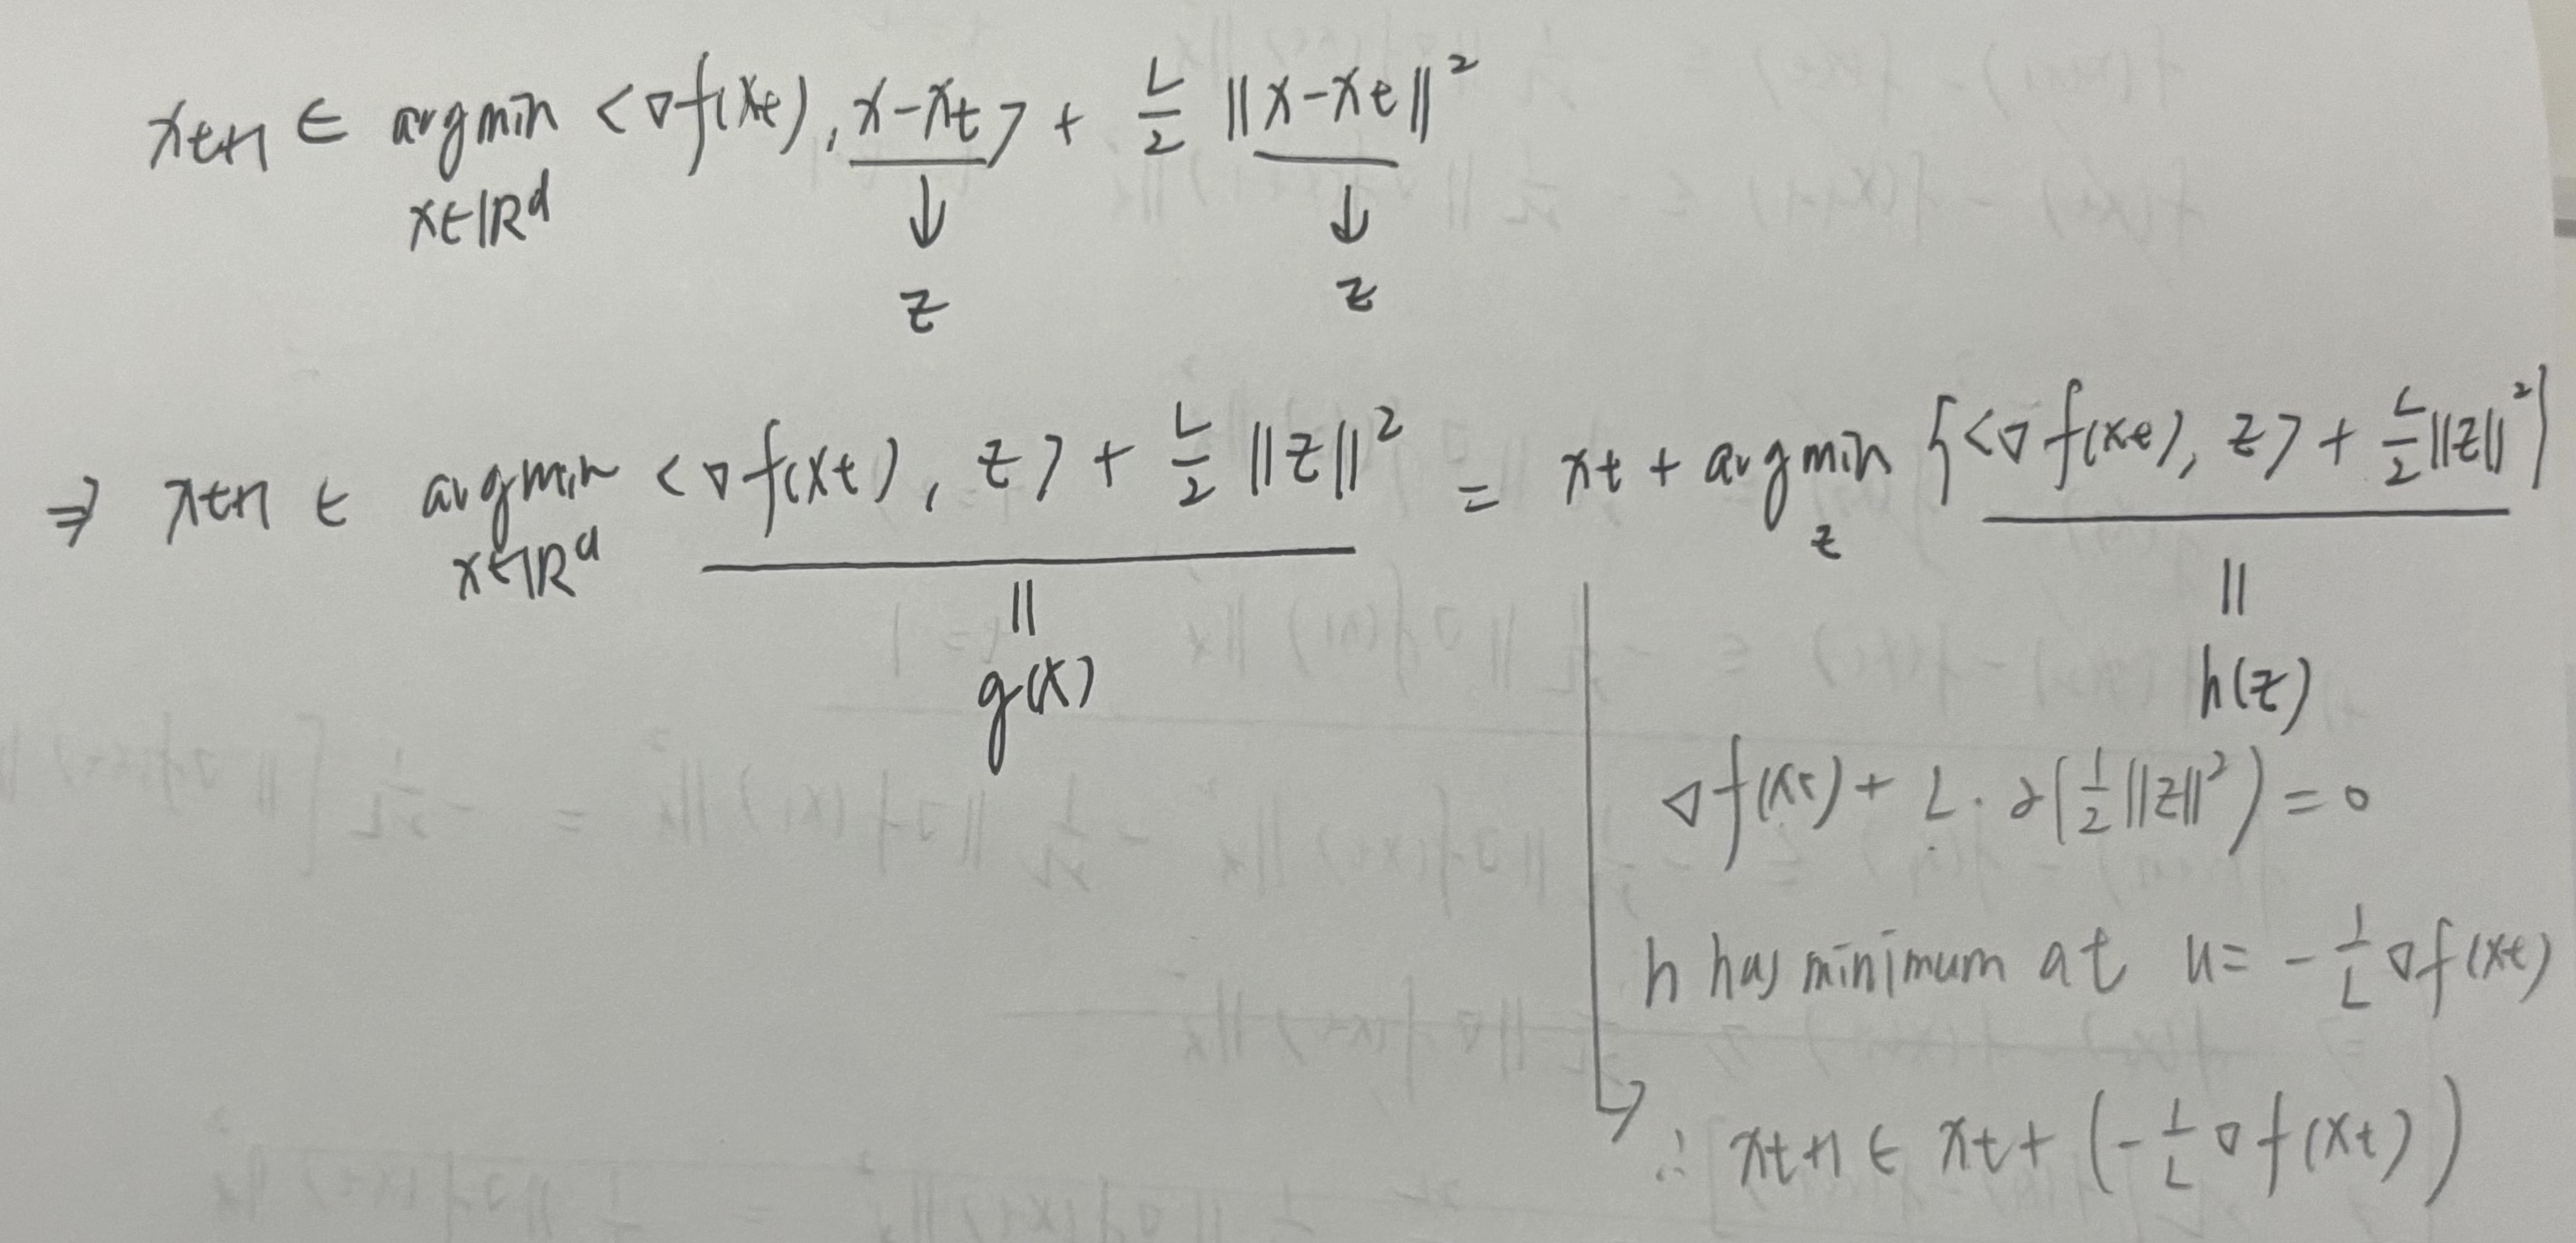
\includegraphics[width=0.7\textwidth]{HW1_images/4_(2).jpg}
\end{figure}

\textcolor{red}{--------------------------------}

Define: 
\begin{align*}
    &\phi: \mathbb{R}^d \to \mathbb{R} \\
    &\phi(z) = \frac{L}{2} \Vert z \Vert^2
\end{align*}

Then the conjugate
\footnote{S. Boyd and L. Vandenberghe, \textit{Convex Optimization}, Cambridge University Press, 2004, p.~91. 
Available online at \url{https://web.stanford.edu/~boyd/cvxbook/bv_cvxbook.pdf}.}
of $\phi$ is defined as:

\begin{align*}
    \phi^*(v) 
    &= \sup_{z \in \mathbb{R}^d} \left( \langle v, z \rangle - \phi(z) \right) \\
    &= \sup_{z \in \mathbb{R}^d} \left( \langle v, z \rangle - \frac{L}{2} \Vert z \Vert^2 \right)
\end{align*}

Let $z = \alpha z'$, where $|\Vert z'\Vert = 1$, then:

\begin{align*}
    \phi^*(v) 
    &= \sup_{z \in \mathbb{R}^d} \left( \alpha \langle v, z' \rangle - \frac{L}{2} \langle \alpha z', \alpha z' \rangle \right) \\
    &= \sup_{\alpha \in \mathbb{R}} \left( \alpha \langle v, z' \rangle - \frac{L \alpha^2}{2} \right) \\
\end{align*}

And by the definition of dual norm, we can derive the inequality (generalization of Cauchy-Schwarz inequality)
\footnote{S. Boyd and L. Vandenberghe, \textit{Convex Optimization}, Cambridge University Press, 2004, p.~637.}
:

\begin{align*}
    \alpha \langle v, z' \rangle \leq \alpha \Vert v \Vert_* \Vert z' \Vert = \alpha \Vert v \Vert_*
\end{align*}

And the original conjugate can be rewritten as:

\begin{align*}
    \phi^*(v) = \sup_{\alpha \in \mathbb{R}} \left( \alpha \Vert v \Vert_* - \frac{L}{2} \alpha^2 \right)
\end{align*}

Taking the derivative:

\begin{align*}
    \frac{d}{d\alpha} \left( \alpha \Vert v \Vert_* - \frac{L}{2} \alpha^2 \right) = \Vert v \Vert_* - L \alpha 
    \implies \alpha = \frac{\Vert v \Vert_*}{L}
\end{align*}

Plugging back in:

\begin{align*}
    \phi^*(v) 
    &= \frac{\Vert v \Vert_*}{L} \cdot \Vert v \Vert_* - \frac{L}{2} \cdot \frac{\Vert v \Vert_*^2}{L^2} \\
    &= \frac{\Vert v \Vert_*^2}{L} - \frac{\Vert v \Vert_*^2}{2L} \\
    &= \frac{\Vert v \Vert_*^2}{2L}
\end{align*}


By Fenchel's inequality
\footnote{S. Boyd and L. Vandenberghe, \textit{Convex Optimization}, Cambridge University Press, 2004, p.~94.}
, which is stated as follows:

\begin{tcolorbox}[greenbox, title = Fenchel's inequality]
    For all $x, y$:
    \begin{align*}
        f(x) + f^*(y) \geq \langle x, y \rangle
    \end{align*}
\end{tcolorbox}

Therefore, we have for all $z, v \in \mathbb{R}^d$:

\begin{align*}
    &\phi(z) + \phi^*(v) \geq \langle z, v \rangle \\
    \Rightarrow \ &\frac{L}{2} \Vert z \Vert^2 + \frac{\Vert v \Vert_*^2}{2L} \geq \langle z, v \rangle \\
\end{align*}

Let $v = \nabla f(x_t)$, and since $z = x - x_t$, which means that choosing the optiaml $z$ is equivalent to choosing the optimal $x$, which is $x_{t+1}$,
so $z = x_{t+1} - x_t$, and we have:

\begin{align*}
    &\frac{L}{2} \Vert x_{t+1} - x_t \Vert^2 + \frac{1}{2L} \Vert \nabla f(x_t) \Vert_*^2 \geq \langle x_{t+1} - x_t, \nabla f(x_t) \rangle \\
\end{align*}

By the result of subproblem $(1)$, and plugging in $y = x_{t + 1}$ and $x = x_t$, we have:

\begin{align*}
    &f ( x_{t + 1} ) \leq f ( x_t ) + \langle \nabla f(x_t), x_{t+1} - x_t \rangle + \frac{L}{2} \Vert x_{t+1} - x_t \Vert^2 \\
    \Rightarrow \ &f ( x_{t + 1} ) - f ( x_t ) \leq \langle \nabla f(x_t), x_{t+1} - x_t \rangle + \frac{L}{2} \Vert x_{t+1} - x_t \Vert^2 \\
    \Rightarrow \ &f ( x_{t + 1} ) - f ( x_t ) \leq \frac{1}{2L} \Vert \nabla f(x_t) \Vert_*^2 + \frac{L}{2} \Vert x_{t+1} - x_t \Vert^2 + \frac{L}{2} \Vert x_{t+1} - x_t \Vert^2 
\end{align*}

\textcolor{red}{--------------------------------}
\begin{comment}
% This part is commented out because we cannot ensure that $\Vert \nabla f ( x_t ) \Vert^2 \geq \Vert \nabla f ( x_t ) \Vert_*^2$

Plugging in $h = \frac{1}{L}$ into $(1)$, the optimal update would be:

\begin{align*}
    &f( y ) = f ( x ) - \frac{1}{2 L} \Vert \nabla f ( x ) \Vert^2 \\
    \Rightarrow \ & f( y ) - f ( x ) = - \frac{1}{2 L} \Vert \nabla f ( x ) \Vert^2 \qquad \text{(plug in } y = x_{t+1}, x = x_t \text{)} \\
    \Rightarrow \ &f ( x_{t + 1} ) - f ( x_t ) = - \frac{1}{2 L} \Vert \nabla f ( x_t ) \Vert^2 
\end{align*}

Thus, to show that $f ( x_{t + 1} ) - f ( x_t ) \leq - \frac{1}{2 L} \Vert \nabla f ( x_t ) \Vert_*^2$ is equivalent to show that:

\begin{align*}
    &- \frac{1}{2 L} \Vert \nabla f ( x_t ) \Vert^2 \leq - \frac{1}{2 L} \Vert \nabla f ( x_t ) \Vert_*^2 \\
    \Rightarrow \ &\Vert \nabla f ( x_t ) \Vert^2 \geq \Vert \nabla f ( x_t ) \Vert_*^2 \\
\end{align*}

By the definition of $\Vert u \Vert_*$:

\begin{align*}
    \Vert u \Vert_* := \underset{x \in \mathbb{R}^d, \Vert x \Vert \leq 1}{\max} \langle u, x \rangle 
\end{align*}

Let $u = \nabla f ( x_t )$, then we have:

\begin{align*}
    \Vert \nabla f ( x_t ) \Vert_* = \underset{x \in \mathbb{R}^d, \Vert x \Vert \leq 1}{\max} \langle \nabla f ( x_t ), x \rangle 
\end{align*}
\end{comment}





\begin{comment}
For any $u, v \in \mathbb{R}^d, \ \lambda \in \mathbb{R}$, we have:

\begin{align*}
    g(\lambda u + (1 - \lambda) v) 
    &= \langle \textcolor{orange}{\nabla f(\lambda u + (1 - \lambda) v)}, \textcolor{Green}{\lambda u + (1 - \lambda) v - x_t} \rangle + \frac{L}{2} \Vert \lambda u + (1 - \lambda) v - x_t \Vert^2 \\
    &= \langle \textcolor{orange}{\nabla f(\lambda u + (1 - \lambda) v)}, \textcolor{Green}{\lambda u} \rangle + \langle \textcolor{orange}{\nabla f(\lambda u + (1 - \lambda) v)}, \textcolor{Green}{(1 - \lambda) v} \rangle - \langle \textcolor{orange}{\nabla f(\lambda u + (1 - \lambda) v)}, \textcolor{Green}{x_t} \rangle \\
    &\qquad + \frac{L}{2} \Vert \lambda u + (1 - \lambda) v - x_t \Vert^2 \\
    &= \langle \nabla f(\lambda u + (1 - \lambda) v), \lambda u \rangle + \langle \nabla f(\lambda u + (1 - \lambda) v), (1 - \lambda) v \rangle - \langle \nabla f(\lambda u + (1 - \lambda) v), x_t \rangle \\
    &= \lambda \langle \nabla f(u), u - x_t \rangle + (1 - \lambda) \langle \nabla f(v), v - x_t \rangle \\
    &= \lambda g(u) + (1 - \lambda) g(v)
\end{align*}
\end{comment}

\subsection*{(3)}

Claim:

\begin{align*}
    \min_{1 \leq \tau \leq t} \Vert \nabla f ( x_\tau ) \Vert_*^2 \leq \frac{ 2 L \left[ f ( x_1 ) - f ( x_{t + 1} ) \right] }{t} , \quad \forall t \in \mathbb{N}
\end{align*}

By the result of the second subproblem, we have:

\begin{align*}
    f ( x_{t + 1} ) - f ( x_t ) \leq -\frac{1}{2L} \Vert \nabla f ( x_t ) \Vert_*^2 \qquad \forall t \in \mathbb{N}
\end{align*}

And since this holds for all $t \in \mathbb{N}$, let $t = 1, \dots, t$:

\begin{align*}
    f ( x_{t + 1} ) - \cancel{f ( x_t )} &\leq -\frac{1}{2L} \Vert \nabla f ( x_t ) \Vert_*^2 \qquad (t = t) \\
    \cancel{f ( x_t )} - \cancel{f ( x_{t - 1} )} &\leq -\frac{1}{2L} \Vert \nabla f ( x_{t - 1} ) \Vert_*^2 \qquad (t = t - 1) \\
    &\vdots \\
    \cancel{f ( x_3 )} - \cancel{f ( x_2 )} &\leq -\frac{1}{2L} \Vert \nabla f ( x_2 ) \Vert_*^2 \qquad (t = 2) \\
    \cancel{f ( x_2 )} - f ( x_1 ) &\leq -\frac{1}{2L} \Vert \nabla f ( x_1 ) \Vert_*^2 \qquad (t = 1) 
\end{align*}

Summing up these inequalities, the terms $f(x_t)$ to $f(x_2)$ on the left hand side will cancel out, and we have:

\begin{align*}
    &f(x_{t+1}) - f(x_1) \leq -\frac{1}{2L} \sum_{i=1}^{t} \Vert \nabla f ( x_i ) \Vert_*^2 \\
    \Rightarrow \ &f(x_1) - f(x_{t+1}) \geq \frac{1}{2L} \sum_{i=1}^{t} \Vert \nabla f ( x_i ) \Vert_*^2 \\
    \Rightarrow \ &\frac{2L \left[ f(x_1) - f(x_{t+1}) \right]}{t} \geq \frac{1}{t} \sum_{i=1}^{t} \Vert \nabla f ( x_i ) \Vert_*^2 \quad \forall t \in \mathbb{N} \tag{1}
\end{align*}

Since:

\begin{align*}
    \min_{1 \leq \tau \leq t} \Vert \nabla f ( x_\tau ) \Vert_*^2 &\leq \Vert \nabla f(x_1) \Vert_*^2 \\
    \min_{1 \leq \tau \leq t} \Vert \nabla f ( x_\tau ) \Vert_*^2 &\leq \Vert \nabla f(x_2) \Vert_*^2 \\
    &\vdots \\
    \min_{1 \leq \tau \leq t} \Vert \nabla f ( x_\tau ) \Vert_*^2 &\leq \Vert \nabla f(x_t) \Vert_*^2
\end{align*}

Summing up these inequalities, we have:

\begin{align*}
    &t \min_{1 \leq \tau \leq t} \Vert \nabla f ( x_\tau ) \Vert_*^2 \leq \sum_{i=1}^{t} \Vert \nabla f ( x_i ) \Vert_*^2 \\
    \Rightarrow \ &\min_{1 \leq \tau \leq t} \Vert \nabla f ( x_\tau ) \Vert_*^2 \leq \frac{1}{t} \sum_{i=1}^{t} \Vert \nabla f ( x_i ) \Vert_*^2
\end{align*}

Plugging this back into $(1)$, we have:

\begin{align*}
    \min_{1 \leq \tau \leq t} \Vert \nabla f ( x_\tau ) \Vert_*^2 \leq \frac{ 2 L \left[ f ( x_1 ) - f ( x_{t + 1} ) \right] }{t} , \quad \forall t \in \mathbb{N} \qquad \square
\end{align*}

\subsection*{(4)}

We're given the algorithm:

\begin{align*}
    &x_1 \in \mathbb{R}^d \\
    &\text{For every }t \in \mathbb{N}, \qquad x_{t+1} = x_t - \frac{\Vert \nabla f(x_t) \Vert_1}{L}\mathrm{sign}(\nabla f(x_t)) 
\end{align*}

where:

\begin{align*}
    &\mathrm{sign}(x) = 
    \begin{cases}
        1 & \text{if } x \geq 0 \\
        -1 & \text{if } x < 0 
    \end{cases} \text{ for any } x \in \mathbb{R} \\
    & \mathrm{sign}(v) = 
    \begin{bmatrix}
        \mathrm{sign}(v[1]) \\
        \vdots \\
        \mathrm{sign}(v[d])
    \end{bmatrix}
    \text{ for any } v = \begin{bmatrix} v[1] \\ \vdots \\ v[d] \end{bmatrix} \in \mathbb{R}^d
\end{align*}

Denote:

\begin{align*}
    \nabla f(x_t) = 
    \begin{bmatrix}
        \frac{\partial f}{\partial x_1}(x_t) \\
        \vdots \\
        \frac{\partial f}{\partial x_d}(x_t)
    \end{bmatrix}
    \in \mathbb{R}^d
\end{align*}

Then:

\begin{align*}
    \mathrm{sign}(\nabla f(x_t)) = 
    \begin{bmatrix}
        \mathrm{sign}(\frac{\partial f}{\partial x_1}(x_t)) \\
        \vdots \\
        \mathrm{sign}(\frac{\partial f}{\partial x_d}(x_t))
    \end{bmatrix}
    \quad, \text{ and }
    \Vert \nabla f(x_t) \Vert_1 = \sum_{i=1}^{d} \left| \frac{\partial f}{\partial x_i}(x_t) \right|
\end{align*}

Note that $l_1$-norm is nondifferentiable, so to find the subgradient, we consider $l_1$-norm in the following form
\footnote{S. Boyd and L. Vandenberghe, \textit{Subgradients}, Notes for EE364b, Stanford University, Winter 2006--07, Apr.~13, 2008. Available at: \url{https://see.stanford.edu/materials/lsocoee364b/01-subgradients_notes.pdf}, p.~5.}

\begin{align*}
    \Vert x \Vert_1 = \{ \max s^Tx \mid s_i \in \{ -1, 1 \} \} 
\end{align*}

And we could find the unique $s$ by choosing $s_i = +1$ if $x_i \geq 0$, and $s_i = -1$ if $x_i < 0$,
this is equivalent to saying that for the case $x = \nabla f(x_t)$, if $\frac{\partial f}{\partial x_i}(x_t) \geq 0$, then $s_i = 1$, otherwise $s_i = -1$,
and we could see that $s$ is actually $\mathrm{sign}(\nabla f(x_t))$.
\bigskip

Thus, the update rule of this algorithm can be rewritten as:

\begin{align*}
    x_{t+1} = x_t - \frac{s^T \nabla f(x_t)}{L} s
\end{align*}

In the second subproblem, we've shown that the optimal update rule is:

\begin{align*}
    x_{t+1} = x_t - \frac{1}{L} \nabla f(x_t)
\end{align*}


\end{document}